% Chapter Template

\chapter{Plan Production and Management} % Main chapter title

\label{chapter:plan_management} % Change X to a consecutive number; for referencing this chapter elsewhere, use \ref{ChapterX}

\lhead{Chapter 4. \emph{Plan Production and Management}} % Change X to a consecutive number; this is for the header on each page - perhaps a shortened title

In this chapter, we introduce the Plan Production and Management layer of our system. Section~\ref{sec:plan_management-intro} introduces the subject, with a review on multi-agent planning, explanation, negotiation and plan management. section~\ref{sec:plan_management-overview} shows the main aspects of this component. Our system is able to use different plan management modalities, as explained in ~\ref{sec:plan_management-modalities}. section~\ref{sec:plan_management-human_knowledge} introduce the idea of maintaing the level of knowledge of a user in a task, which will be used both in plan generation and management. section~\ref{sec:plan_management-plan_generation} introduces our task planners, HATP (\ref{subsec:plan_management-hatp}), and HAPP (\ref{subsec:plan_management-happ}), and shows how plans are adapted to the expertise of humans in the  tasks (\ref{subsec:plan_generation-adapting_knowledge}). section~\ref{sec:plan_management-plan_explanation} shows how plans are explained to users, and section ~\ref{sec:plan_management-negotiation} how they are negotiated.  section~\ref{sec:plan_management-plan_manager} introduces the plan management aspects of this layer. We developed different strategies, shown in subsections ~\ref{subsec:plan_management-sequential_plan_management} and ~\ref{subsec:plan_management-adaptive_parallel_plan_manager}. section~\ref{section:plan_management-plan_monitoring} shows how are system is able to monitor human actions and task. Finally section~\ref{sec:plan_management-experiments} details a user study created to evaluate the ability of our system to adapt to users.


\section{Introduction}
\label{sec:plan_management-intro}
\subsection{Cooperation between agents}
Robots can be used to perform a large number of different operations. Some of these will be simple enough that the robot can just achieve its task by performing a prefixed sequence of elementary actions. In other cases, the robot might have to achieve complex goals, which require the ability to create plans and to adapt them to the current state of the world. When cooperating with other agents, the robot has to build a shared plan, which includes the actions that every agent need to perform, in order to coordinate and ensure the corrent achievement of the goal. We can imagine the following process:
\begin{itemize}
	\item The system receives a new goal. This can be directly introduced by a human, or chosen after some kind of reasoning by the robot.
	\item One of the agents (the robot or the humans) proposes a shared plan to achieve the goal, and presents it to the other agents.
	\item The agents negotiate the plan. In some situations, one of the agents might not be able (or might not want) to perform a specific action, or sequence of actions. The agent can refuse the plan, proposing a correction or a completely different plan.
	\item The agents execute the plan. Each agent performs its part of the plan. In addition, agents may check the state of others to monitor the correct execution of their part of the plan or to cordinate with them.
	\item An agent might fail its part of the plan. If this happens the agents need to create a new plan to account for this failure.
 	\item The process continues until the goal is achieved or it becomes unachievable (for example, a needed resource is no longer available).
\end{itemize} 
When humans cooperate this process can be very quick. For simple tasks humans are able to coordinate without explicitly forming a plan, in particular if they are used to cooperating together. Other times, when there are unexpected problems during the execution of a plan, humans are able to quickly readapt their plan, without completely restarting this process. In order to cooperate in a natural way with humans, robots need to reproduce these mechanisms.

\subsection{Multi Agent Planning}
Multi-Agent planning   is an important and studied topic in the AI community \cite{durfee1999survey}. There are several approaches to this problem, using classical or probabilistc planning. There are several issues to consider:
\begin{itemize}
\item Localized vs Centralized. A multi-agent planner might be localized, meaning that separate systems plan independently and then communicate to build a shared plan (an idea investigated, for example in \cite{nikolaidis2013cross,guestrin2002distributed} ); or centralized, meaning that a single system plans for all the agents.
\item Coordination. Agents need to coordinate their plans, in particular in the presence of shared resources. Imagine, for example, two agents, Max and Bob, that are using a tool to repair a set of cars. If Max is proceeding faster than Bob and the two do not coordinate, Max might take the tool and leave, starting to repair another car, ignoring the fact that Bob still needs the tool. This example shows that it is important to reason on the duration of actions performed by agents. At the simplest level, agents need to know the advancament of the sub-plan of other agents. More complex reasoning might take into account how long an agent needs to perform a certain sub-task, in order to refine a plan. 
\item Cooperation. Even when performing different sub-tasks of the same plan, agents can help each other, for example by passing items, thus improving the efficiency of the plan. Multi-Agent problems can be loosely or tightly coupled, depending on the quantity of interactions between agents. \cite{torreno2015approach} propose a general purpose approach able to plan at differet level of coupling.
\item Communication and Knowledge. In a multi-agent environment each agent might have an incomplete or incorrent belief on the world, which might lead to wrong or sub-optimal actions. Agents may communicate to progressively build a correct belief model on the state world. 
\end{itemize}

Several approaches has been studied to bring the multi-agent planning problem in a probabilistic framework. \cite{boutilier1999sequential} create a centralized MDP, able to select at each time step actions for every present agent. Dec-POMDP \cite{bernstein2002complexity} and I-POMDP \cite{gmytrasiewicz2005framework} are more complex frameworks, that take into account the belief models of agents. The complexity of these models makes them difficult to use in even moderately difficult scenarios. A solution to this problem is considering simpler problems, where the agents mostly work independently and interact only in limited situations, such as in \cite{melo2013heuristic}.  Unfortunately this solution is not feasible in the kind of scenarios that we are interested in, where robots and humans work in a straightly coupled manner. 

\subsection{Plan Explanation and Negotiation}
In order to form  shared plans, agents often communicate, explaining tasks to each other and negotiating to agree on a solution. In \cite{Lallee2013} the authors suggest that joint plans should be fully communicated in order to sustain effective collaboration. 

Some authors have started to investigate this topic in robotics. In \cite{Petit2012}, a human is able to teach new plans to a robot verbally through ``spoken language programming''. \cite{Sorce2015} studies the inverse problem, where the system is able to explain plans to users. 

In a collaborative scenario, all the agents must agree on the shared plan. If there is a disagreement the agents might negotiate to find a nother solution.  This problem has been studied, for example, in \cite{fabregues2014hana}, where the authors present the HANA system, an architecture that allows robotic and human agents to negotiate in competitive and cooperative settings.

\subsection{Plan Management}
Finally, the shared plan needs to be executed. Agents need to perform their part of the plans and to monitor their partners in order to coordinate with them. Two examples of systems able to execute shared plans are  Chaski \cite{shah2011improved} and Pike \cite{karpas2015robust}. Chaski is also able to execute plans in two different modalities: equal partners or leader and assistent.

\section{Overview}
\label{sec:plan_management-overview}
Our system presents a planning layer which is able to perform the following tasks:
\begin{itemize}
	\item Interface with external planners in order to create a shared plan. The system has been integrated with a HTN (Hierarchical Task Network) based planner, HATP (Human-Aware Task Planner), and with a multi-agent MDP planner.
	\item Explain a plan to human agents. Depending on the human expertise on the tasks to be performed, the robot will adapt the explanations, focusing more deeply on tasks that agents do not know how to perform. This idea is supported by research on Intelligent Tutoring Systems \cite{brusilovskiy1994construction}  and on e-learning \cite{brusilovskiy2005}, which  prove the necessity of keeping and updating a model of the learner's knowledge to efficiently teach a task.
	\item Negotiate a plan. Our system has some simple mechanics allowing a human to reject a plan, specifying which parts of it he does not want to perform. The robot will take the human's preference into account when producing a new plan.
	\item Monitor a human plan. Our system is able to monitor other agents' parts of a plan, to cordinate with them and to react when an agent fails an action or his actions diverge from the current plan.
	\item Receive plans from a user. Users can interact with the robot with a tablet application, asking it to execute specific actions or goals.
	\item Executing shared plans in different modalities. The robot can be a leader, assistant, or equal partner of humans during plan management.
\end{itemize}

A number of modules implement this ideas, as shown in figure \ref{fig:plan_management-architecture}:
\begin{itemize}
\item Task Planner. Creates a shared plan for the involved agents.
\item Plan Explanation. Explains the plan to the involved agents, adapting it to their knowledge.
\item Plan Negotiation. Negotiates the plan with the involved agents.
\item Plan Management. Manages the current plan, interacting with the Execution Management layer to execute the robot's action and with the Situation Assessment layer to monitor human's actions.
\end{itemize}

After receiving a goal from the Goal Management layer, the Plan Management module sends a request to the Task Planner to look for a suitable plan. If there is a plan, depending from the current modality, it will activate the Plan Explanation and Plan Negotiation modules to communicate with the involved humans, or directly start executing it. If the plan needs to be negotiated this process is repeated. When a plan is agreed by all the agents, the Plan Management module starts executing it. 

\begin{figure}[ht!]
	\centering
	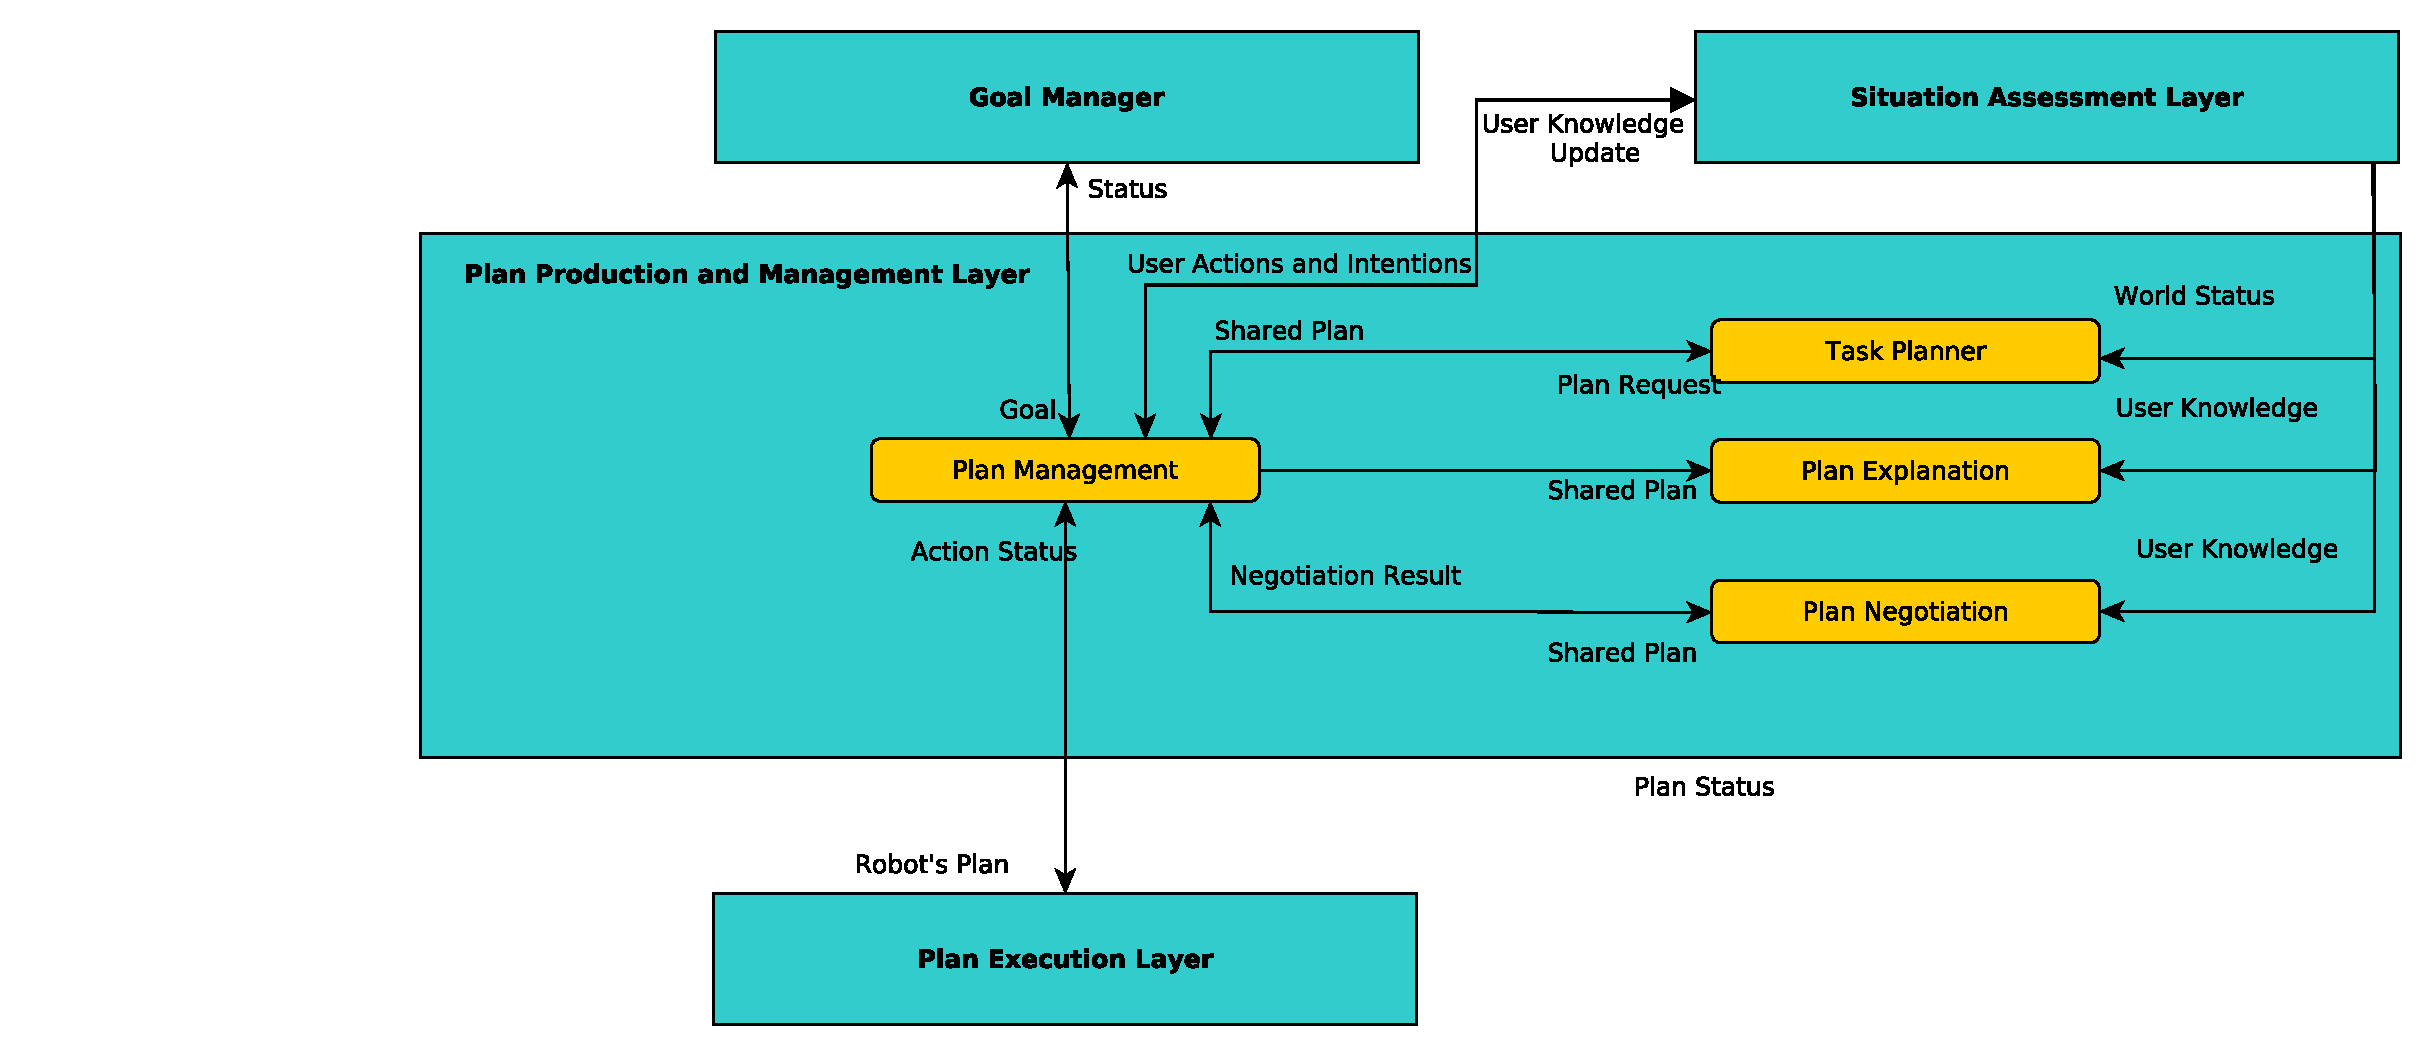
\includegraphics[scale=0.5]{img/plan_management/architecture.pdf}
	\caption[The architecture of the Plan Production and Management layer]{The architecture of the Plan Production and Management layer. Light green rounded rectangles represent modules, while dark green rectangles layers. Arrows represent message exchanged between components, with the label detailing the message.}
	\label{fig:plan_management-architecture}
\end{figure}


Part of this chapter was presented in \cite{Lallement2014,milliez2016using,fioreiser2014}.

\section{Plan Management Modalities}
\label{sec:plan_management-modalities}
When acting together, agents sometimes do not have the same decision power, with one of them assuming the role of a leader. We represent this idea, in our system, by proposing three different modalities: \textit{robot leader}, \textit{human leader}, and \textit{equal qartners}. The robot is able to switch from one modality to another during the execution of a plan. For example, if the current modality is \textit{robot leader} and the Robot receives a command from a user, it will switch to the \textit{human leader} modality, after interrupting its current action.

\subsection{Robot leader}
In this modality the robot, after computing the plan, will explain it, negotiate it and start executing it.
The robot will track the status of humans, informing them of which actions they should execute. This modality can be helpful when interacting with  naive users or in tasks where the robot has a better knowledge of the
domain or of the environment than the other agents.

\subsection{Human Leader}
The human can also create plans, interacting with the robot by using a
tablet application, as explained in section \ref{sec:situation_assessment-communication}. In this modality the robot   
will simply observe the surroundings and wait for user inputs. This modality is always available and has a priority over
the other two modalities. If the robot receives a command from the
application while it is in another modality, it will abandon its current
plan, stopping its actions at a safe point, and then execute the users'
command. We feel that this interaction modality is important for two
different reasons.  First, some users will simply prefer to be in
charge of the execution process, for a matter of personal preference or because they
feel they have a deeper knowledge on how to realize the current task
than the robot. We can picture, for example, industrial or medical
scenarios, where the human is the leader and asks the robot to perform
different tasks to help him, when needed. A second use of this modality is in situations where
the robot does not have  a clear estimation of the users' intentions and
goals. For example, in a domestic environment, a user could decide to
order a robot to bring him a drink, a need that the robot can not always anticipate.

\subsection{Equal Partners}
In the last presented operation modality the robot will try to help
the human to complete a task. At the start of the scenario, the robot
will stand still and observe the environment. After the user takes an
action the robot will calculate a plan and try to help as it can, by
performing actions related to that task and by giving helpful information to
the user, for example to fill gaps in their knowledge. In this modality, 
the robot will not explain or negotiate the current plan and will not warn humans if
their actions differ from the plan computed by the robot.

We feel that, particularly in non-critical tasks, where defining an accurate plan between the partners is not
fundamental, this modality is a very natural way of
interaction between different partners.



\section{Plan Generation}
\label{sec:plan_management-plan_generation}
One of the goals of our system is flexibility; we consider important the possibility to interface with external components. We built an intermediate Plan Generation module that interacts with external planners,  returning  plans represented in a common format that can be handled by the other modules. 

In particular, we require that each planner produces an HTN tree of tasks, showing the decomposition of the plan, which will be helpful in the explanation and monitoring phases; and a set of streams, one per agent, which is useful during the execution of the plan. We introduce casual links between actions, even of different streams, to ensure synchronization. A casual link $l=(a_1,a_2)$ indicates that action $a_1$ should be execute before action $a_2$. This ensures that all the preconditions to execute $a_2$ are fullfilled. Moreover, if $a_1$ and $a_2$ are executed by different agents, and if there is a shared resource connected to the action, the casual link indicates that the resource will be released by the agent only after $a_1$ is completed. An example of these data structures is shown in figure~\ref{fig:plan_management-plan_structure}.

\begin{figure}[ht!]
 \centering
  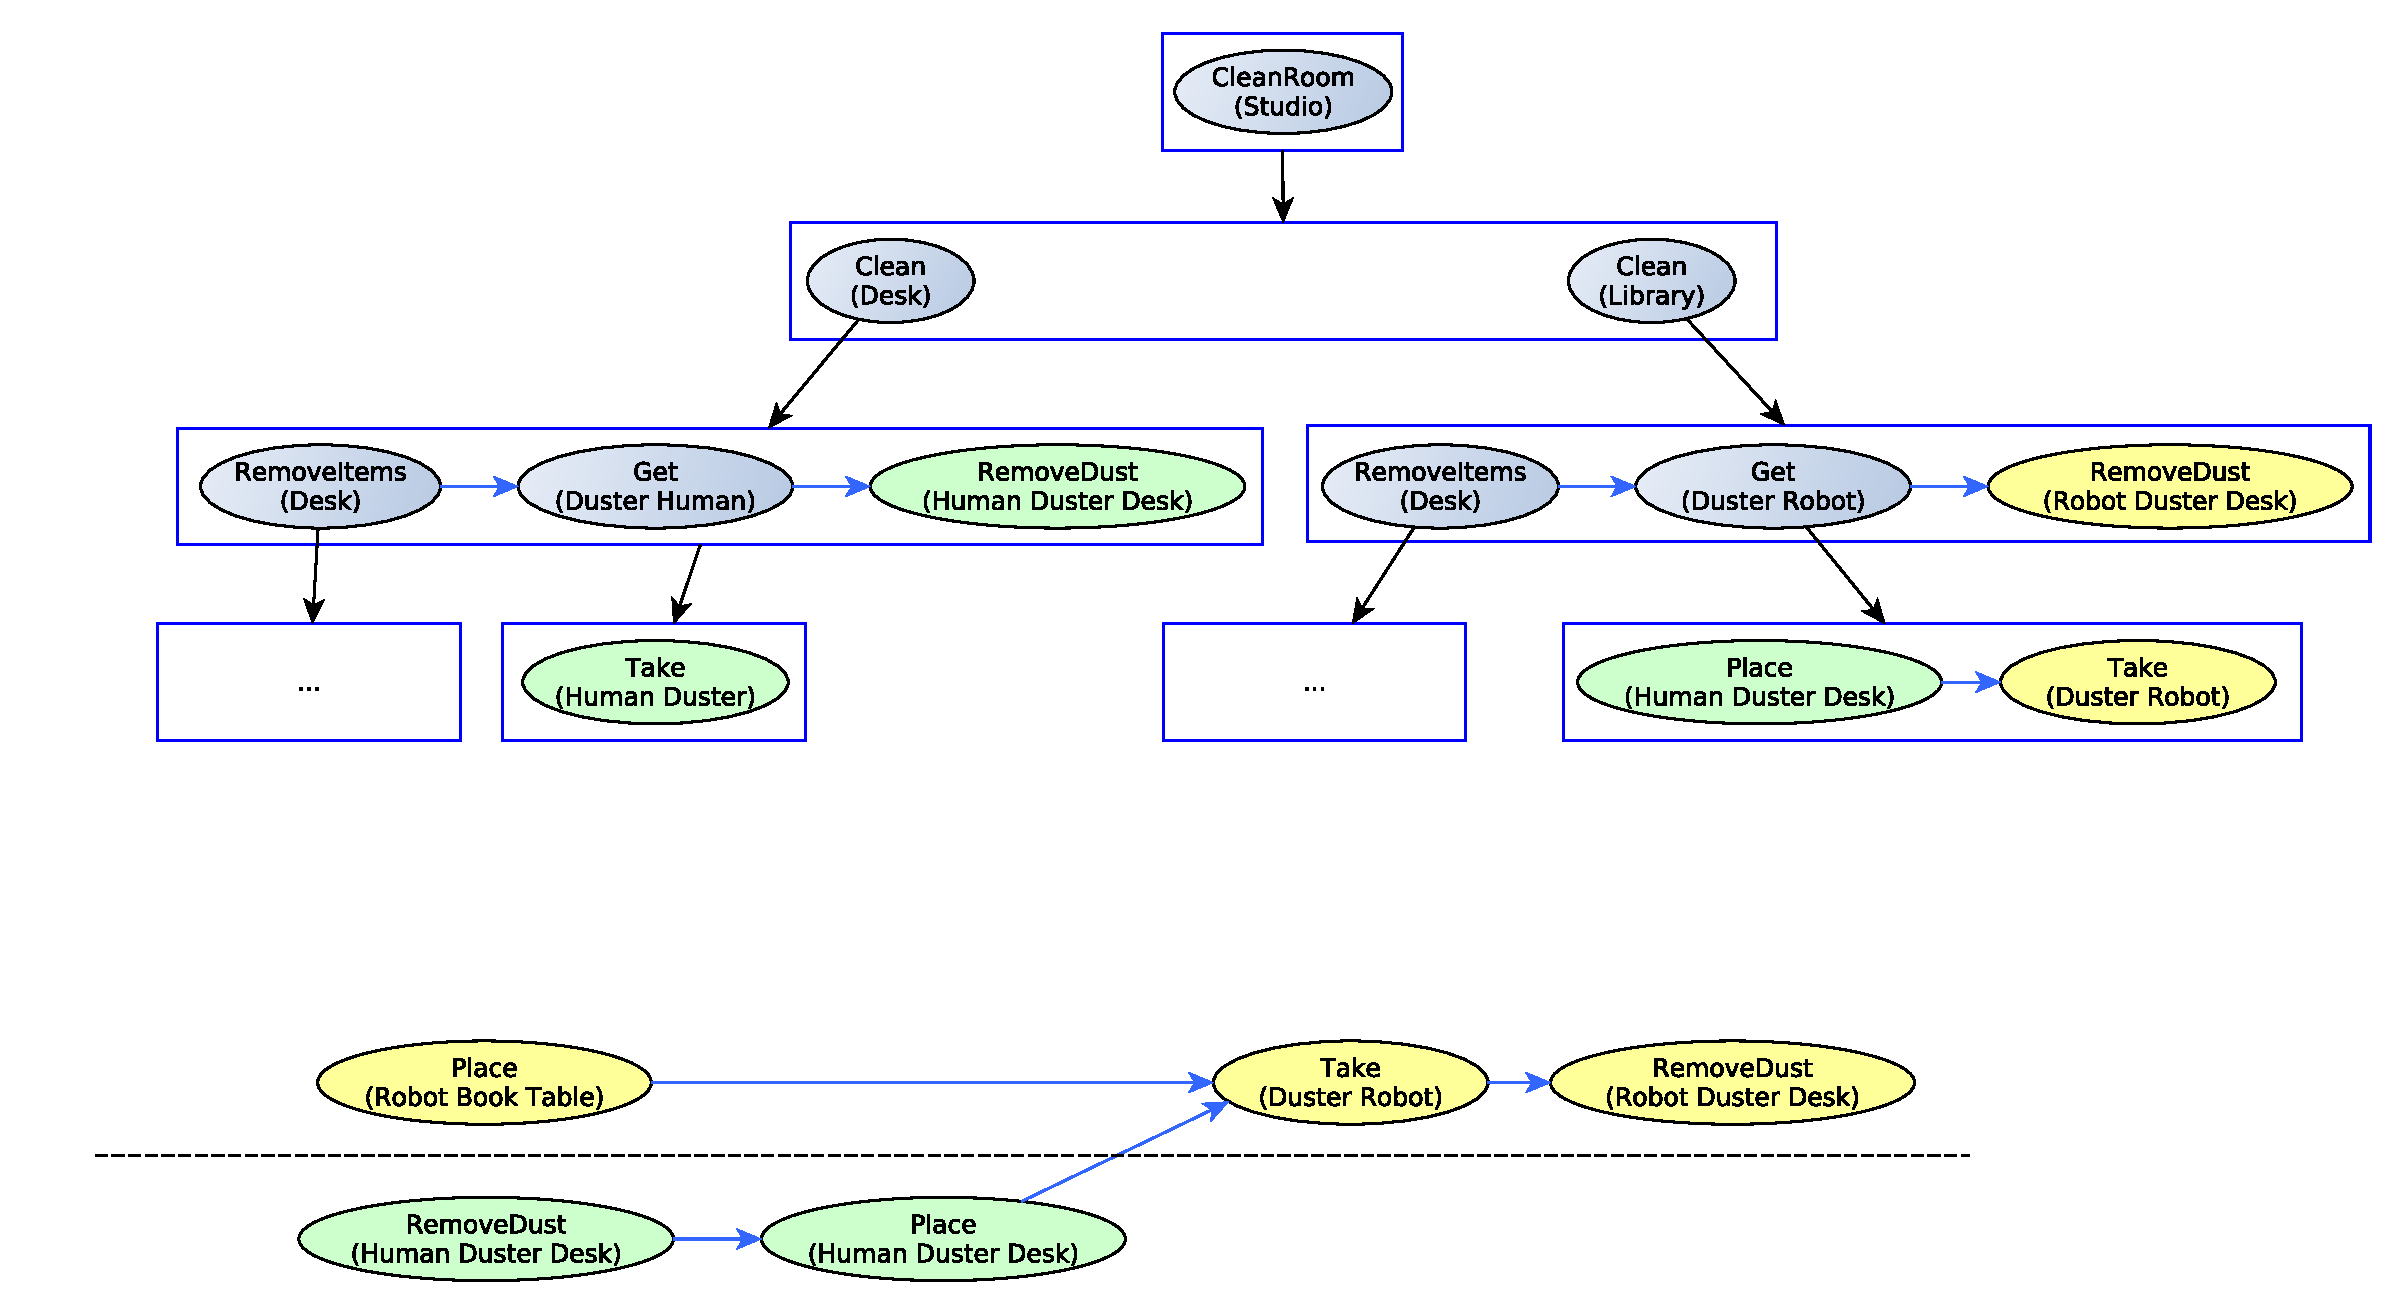
\includegraphics[scale=0.45]{img/plan_management/plan_data_example.pdf}
 \caption[Plan data structures]{a) A HTN plan data structure used in our system, representing a possible way to clean a room
 with two agents, a robot, and a human. Blue ellipses represent tasks, green ellipses represent
 actions assigned to the human, and yellow ellipses actions assigned to the robot. Each decomposition is grouped
 in a blue rectangle. Black arrows link a method to its decomposition, while blue arrows represent casual links. The two squares with a "..." label represent decompositions that are not shown in this picture.
 b) A part of the plan streams associated to the tree data structure. The upper stream represents the robot, and the lower one a human. Notice the casual link between the Place(Human Duster Desk) in the human stream and the Take(Robot Duster) in the robot stream. This link indicates that the robot should wait that the human places the duster before executing the action to take it, ensuring synchronization }
 \label{fig:plan_management-plan_structure}
 \end{figure}


At the moment, we tested two different planners with our system, which will be shown in the next subsections.


\subsection{Human-Aware Task Planner}
\label{subsec:plan_management-hatp}
Computing a plan in complex environments can be very hard and time consuming. A useful approach to reduce the search space in planning is introducing the knowledge of an expert in the system, in order to guide the planner toward desirable states. An implementation of this idea is HTN, where the domain expert specifies a hierarchical library of operations, called methods, when the operation is a node in the hierarchy, and actions, when the operation is a leaf. HATP is a planning framework that extends HTN for human-robot interaction tasks. Among the capacities of HATP we can find:
\begin{itemize}
\item Multi-Agent. HATP is able to plan for different agents at the same time, humans and robots. The planner can also compute ``joint actions", that involves more agents at the same time.
\item Social Rules. The domain expert can introduce a set of rules, which represent desirable behaviors, for example to distribute in different ways operations between agents, or to avoid specific sequences of actions.
\item Cost Driven. The domain expert can specify a cost for actions. Plan pruning allows to explore more efficiently the search space, discarding paths that are not promising.
\end{itemize} 

Plans are represented as an HTN tree decomposition and as a set of streams, one per agent, which shows which actions each agent needs to perform. Casual links are introduced between streams to ensure synchronization.

% \section{Plan Negotiation}
% \label{sec:plan_management-negotiation}
% Once the robot has presented the plan to his collaborators, it can start a negotiation phase. 

% We introduce a simple negotiation algorithm, that starts with the robot asking humans for approval of the plan, inquiring what is wrong in case of disagreement. We handle two different human requests. First, the user can express his preferences, either to perform a task previously assigned to the robot or to not perform a task assigned to him. The other possibility is to inform the robot that the user cannot perform an action. The system will store these information and try to find a new plan, taking them into account, before starting a new explanation and negotiation phase.
 

\section{Plan Management}
\label{sec:plan_management-plan_manager}

Once the plan has been accepted, the agents can start executing it. The three different plan management modalities presented imply different strategies.


\subsection{The robot is not leader}
\label{subsec:plan_management-robot_not_leader_manager}
In the \textit{human leader} and \textit{equal partners}  modalities the robot should not interfere with the actions of its partner. The Plan Management algorithm will be divided in different threads of execution, one for each agent. We will now explain this algorithm, which is shown in figure \ref{fig:plan_management-manage_plan_not_leader}.
\begin{itemize}
  \item Each thread executes the part of the plan of an agent, composed by $n$ different actions.
  \item For each action, for every casual link $(a_i,a_n$), where $a_n$ is the current action, and $a_i$ is another action, the plan manager waits until $a_i$ is completed, or there is an error. This is handled in the \textit{waitCasualLinks} procedure.
  \item When all the casual links have been satisfied, the execute\textbackslash monitor procedure is called, depending if the thread is managing the robot or another agent. The \textit{executeAction} operation interacts with the Execution Management layer to complete the action, while the MonitorAction operation with the Situation Assessment layer.
  \item If these procedures succed, the plan manager switches to the next action, otherwise it returns a failure.
  \item The process is continued until there is a failure or the plan for the current agent is completed.
\end{itemize} 

\begin{figure}[ht!]
 \centering
 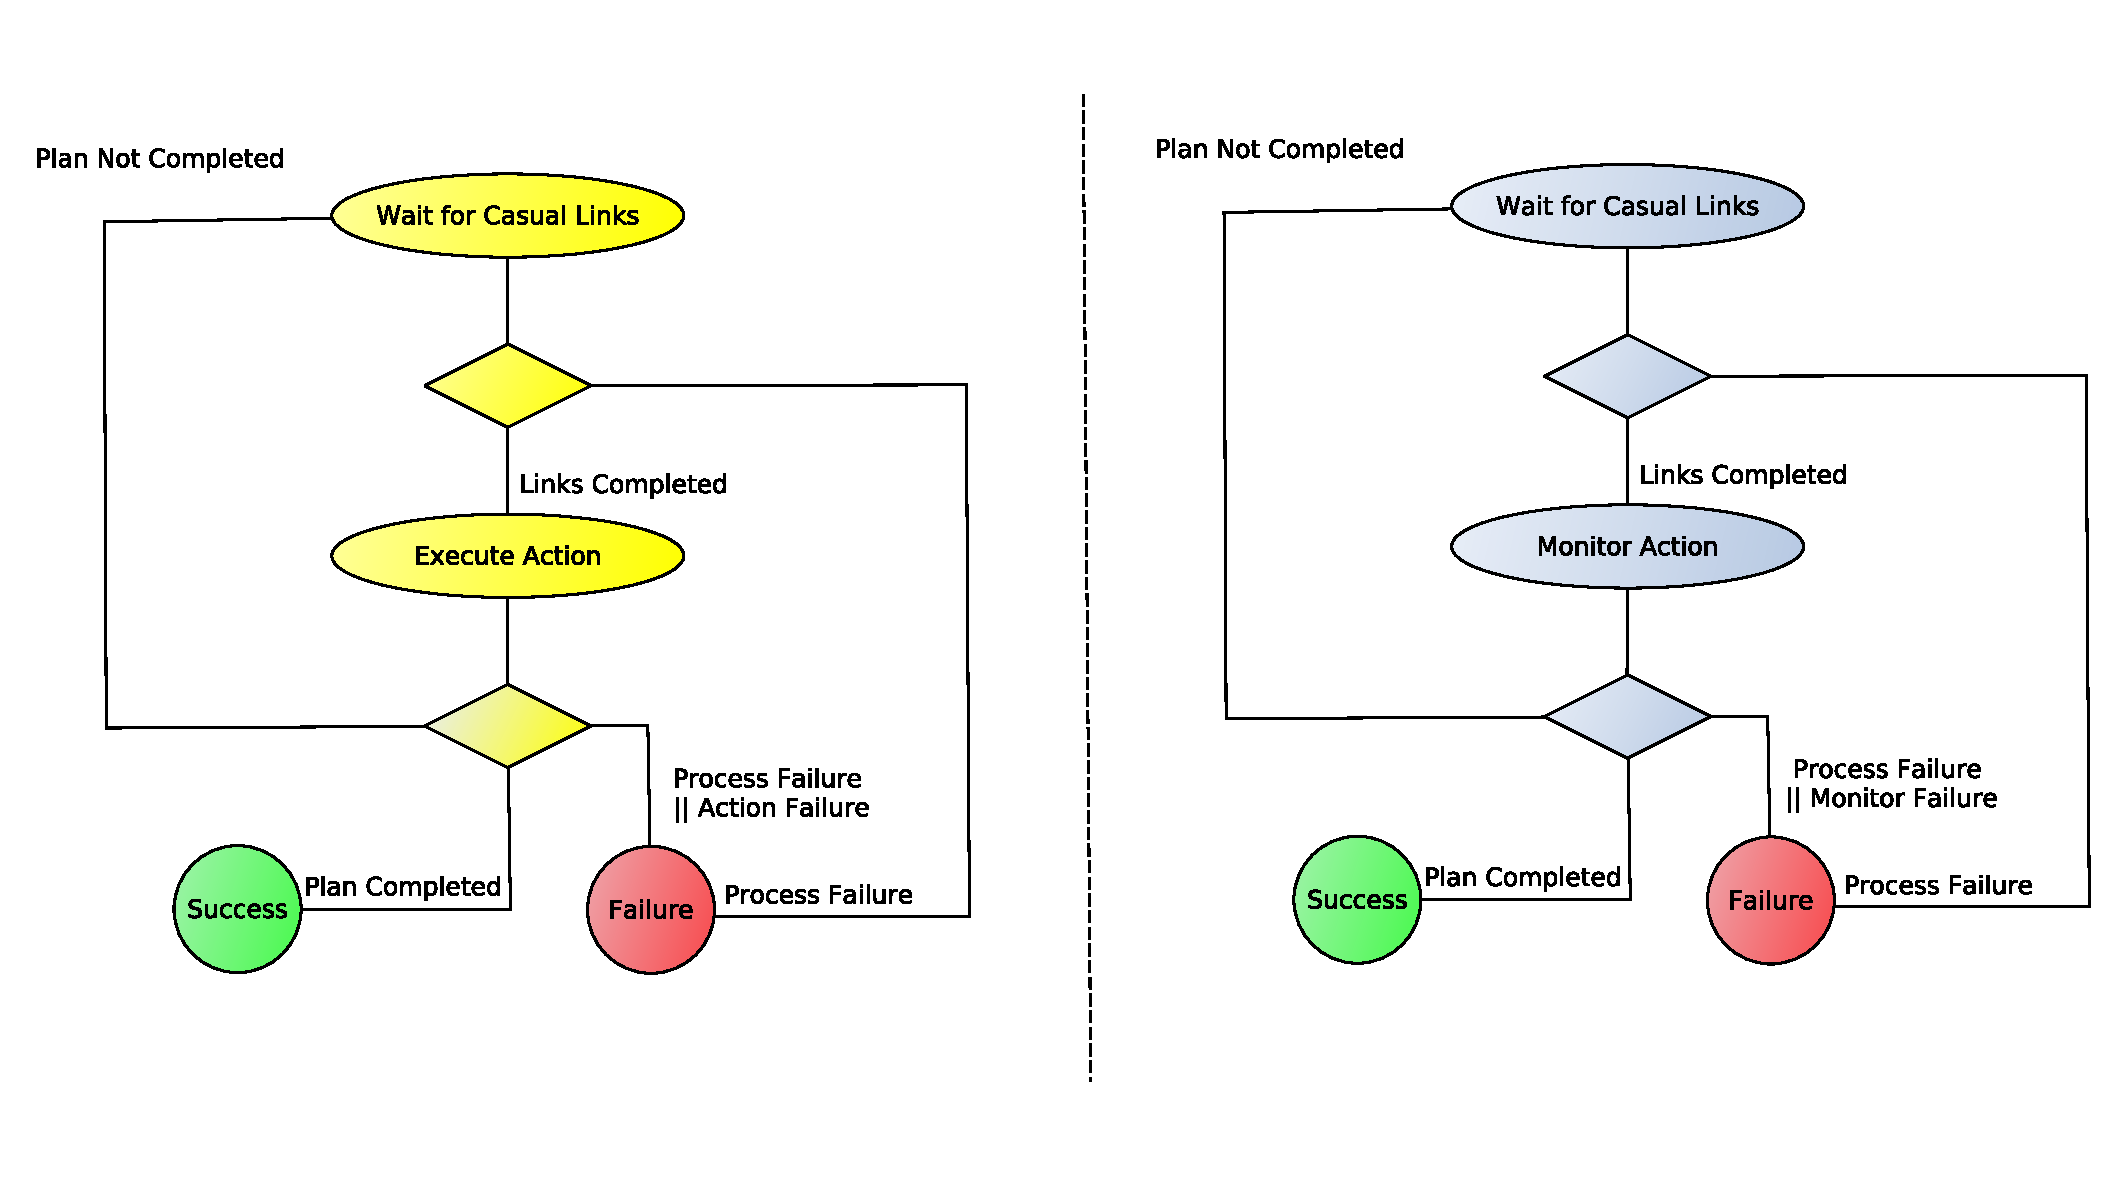
\includegraphics[scale=0.6]{img/plan_management/manage_plan_not_leader.pdf}
 \caption[Plan Management when the robot is not leader]{The plan management algorithm used when the current modality is not \textit{robot leader}. The algorithm is composed by different threads, one for each agent. In this instance, the upper lane represents the robot's management thread, while the bottom a human's management thread. Elliptic nodes represent operations. Diamond nodes, representing divergences in the algorithm, where adding only when they could simplify the understanding of the algorithm. Arrows imply a transition between nodes, with the label of the arrow representing the condition of the transition, when present. The absence of a label implies that a transition is always applied. The blue circle node, called ``start", represents the start of the algorithm. The green and red circle node, instead, represent the success or failure of the algorithm.}
 \label{fig:plan_management-manage_plan_not_leader}
 \end{figure}

Failures in the algorithm lead to a replan request. If a new plan is found, the algorithm starts again, otherwhise the goal is considered failed.

\subsection{The robot is leader}

In the \textit{robot leader} modality the situation is more complex. The plan needs to be analyzed and potentially integrated with ``explanation actions", used to explain a task to a human. In the plan management algorithm previously explained, the robot expects the human to perform a specific stream of operations, and will replan when he deviates from this stream. In this modality, the robot will expect users to execute a specific set of tasks, warning them if they do not respect this allocation. Sometimes, the robot will choose the decomposition of the tasks that should be executed by a user, but, when the partner is competent enough in a high-level task,  we may want to allow him the flexibility to execute it as he sees fit. 

In this situation, we would like to use information about the task allocation, created in the planning\textbackslash presentation\textbackslash negotiation phases, to avoid to replan when a user is executing a task where we allow him flexibility in a different way from the strategy planned by the robot.  Unfortunately, this approach poses several problems. In fact, there might be conditional dependencies between actions of the robot and of the human in the original computed plan. If the human follows another set of actions, the coordination process might break. There are different solutions to this problem:
\begin{itemize}
	\item Executing the plan in a sequential way, disallowing parallelism between the agent. This strategy is less efficient, but it might be useful when the robot wants to teach a task to a user.
	\item Not allowing freedom of execution in tasks whose children have conditional links to robot actions. 
	\item Executing the plan while allowing the user to deviate from it, and repairing it when needed. This approach poses different problems. The first one is understanding when a deviation from the plan imposes the necessity of a repair. The second is that the task planner might generate a plan with a different task allocation, which implies that the robot should restart the explanation process.
\end{itemize}

In \cite{milliez2016using} we presented a first version of an adaptive plan management algorithm, based on executing a plan in a sequential way. We present this algorithm in the following subsection, and then introduce a new parallelized version of it, based on plan reparation.



\section{Plan Monitoring}
\label{section:plan_management-plan_monitoring}

\subsection{Introduction}
During the execution of a plan, the robot will monitor other agents. In general, having a shared plan, the robot knows what is the user's next expected action, and can monitor if it is accomplished. Plan monitoring poses a number of different issues:
\begin{itemize}
\item Understanding when the next expected action has been performed. In some situations the robot will monitor the execution of a specific action. In this event, it needs to understand when the action has been completed.
\item Understanding when the next expected task has been performed. In some situations, the robot wants to give a human cooperator the freedom to perform a subtask has he sees fit. This is a more complex problem than monitoring a specific action, since the robot needs to reason on the results of sequences of actions.
\item Evaluating the human engagement in the current task. The robot needs to understand if the human is trying to accomplish its current task, if he momentarily interrupted it, or if he abandoned it.
\end{itemize}

\subsection{Monitoring Plans}
When executing a shared goal, the Plan Production and Management layer needs to interact with the Intention and Action Recognition module in the Situation Assessment layer. Normally, this module is not able to monitor joint goals, since the inference mechanism presented in subsection \ref{sec:situation_assessment-action_evaluation} is based on single-agent MDPs. To solve this issue, while performing a shared plan, we create, in the Situation Assessment layer, a new intention for each node in the HTN tree whose task can be currently performed (meaning, if it has casual links to other tasks, they have already been satisfied). We associate to these intentions the linked MAMDP, as previously explained in \ref{subsec:plan_management-happ},
 and the context node \textit{have a shared plan}, which is treated as evidence with a true value. We call these intentions \textit{plan intentions}.

We associate to each known intention a precomputed \textit{expected length}, which is the expected time to accomplish the linked goal.

The robot can be updated at each time on what actions have been performed, using the mechanisms described in section \ref{sec:situation_assessment-intention_recognition}. This way, the robot can compare actions that are actually performed by humans with those that \textit{should} be performed following the shared plan.

Using the Intention and Action Recognition module, the robot can infer which is currently the most likely human intention. If the current intention equals the task to monitor, the robot infers that the human is actively working to complete its task. We consider the task, and the monitor procedure, as completed when the linked MAMDP reaches a goal state.

If the human is currently not involved in the monitored task there are three possibilities:
\begin{itemize}
	\item The human has momentarily interrupted the task. This can be inferred if the human is currently involved in another intention, which does not belong to the \textit{plan intentions}, and whose expected length is \textit{short}. In this case, the monitor procedure will not return an error until a predefined \textit{allowed time}.
	\item The human has abandoned the task.  This can be inferred if the human is currently involved in another intention, which does not belong to the \textit{plan intentions}, and whose expected length is \textit{long}. The monitor will return a \textit{not involved error}. 
	\item The human is performing another task in the shared goal. This can be inferred if the human is currently involved in another intention, which belongs to the \textit{plan intentions}. In this case the monitor will return an \textit{other task error}. 
\end{itemize}


\subsection{Monitoring and Unseen Actions}
Often, in cooperative tasks, agents will operate in different locations, and so they can not observe each other actions all the time. Perhaps one of the agents is cooking in the kitchen,  while the robot is preparing the table for dinner. While we do not deal, in this work, with these issues, there are several studies on plan recognition in partially observable environments, like \cite{geib2005partial}.
